\documentclass[11pt]{article}
\usepackage{amsmath}
\usepackage{amssymb}
\usepackage{amsthm}
\usepackage{amscd}
\usepackage{amsfonts}
\usepackage{fancyhdr}
\usepackage{graphicx}
\usepackage{sectsty}
\usepackage{subfig}
\usepackage{epstopdf}
\graphicspath{{../../../figures/},{../../../images/}}

%\textwidth6in

%\sectionfont{\fontsize{12}{15}\selectfont}

%\setlength{\topmargin}{0in} \addtolength{\topmargin}{-\headheight}
%\addtolength{\topmargin}{-\headsep}

\pagestyle{fancy}\lhead{Robert F.K. Martin Thesis Proposal} \rhead{May 2018}
\chead{{\large{\bf }}} \lfoot{} \rfoot{} \cfoot{\thepage}

\newcounter{list}

\begin{document}
\bibliographystyle{IEEEtranS}
%\bibliographystyle{hunsrt}
\newpage
\thispagestyle{empty}
\pagenumbering{gobble}
%\begin{spacing}{1}
\begin{center}
\vspace{\stretch{2}}
\textbf{VISUAL MONITORING OF SUBTLE HUMAN MOTION}\\
\vspace{\stretch{1}}
Ph.D. Thesis Proposal\\
\bigskip
Robert Francis Kennedy Martin\\
\end{center}
%\end{spacing}
\clearpage
\pagenumbering{arabic}
\section{Abstract}
\noindent
Observation plays a key role in the assessment of medical patients. It is the focused and attentive study of a person or situation. From the initial visit to a follow-up examination, a doctor’s visual inspection is as important as any diagnostic test. There are many illnesses that can only be diagnosed through observation and directed questioning, especially in the psychiatric domain. Visual observations can be less reliable than diagnostic tests due to human error, subjective measurement, or lack of attention. With the availability of cheap cameras and computer storage, many of these observations are now being recorded. But due to the time-intensive nature of video analysis, the full potential of these videos has not been realized. With recent advances in computer vision, new and powerful techniques can be applied to videos to look for descriptive behaviors that indicate certain pathologies. By having these videos automatically processed, not only can they be used for initial diagnosis, but for evaluating the efficacy of therapeutic solutions as well. This thesis will introduce techniques and metrics to observe specific behaviors towards the goal of analysis for psychiatric patholgies.
\section{Introduction}
\noindent
One of the first and most important steps in a physical examimation is inspection. This is a crucial piece of the initial doctor/patient interaction as it gives important clues to the initial diagnosis and provides a starting point for further investigation and questions. Additionally, initial observations can be used as a baseline for follow-up interactions. Visual inspections are an especially important part of many psychiatric examinations, as emotional attitudes, facial expressions, and words or silence may indicate different manifestations of a mental disorder. Among the many psychiatric disorders that fall into this category, some of the more well-known are attention-deficit hyperactivity disorder, obsessive-compulsive disorder, Tourette's syndrome, depression, and post-traumatic stress disorder.

Human observation is inherently imperfect and subject to many sources of error. One of the first rules  is objectivity; confirmation bias can lead to many observations either being missed or ignored. Observations must be focused. Even the smallest lapse in attention can miss some imortant behavior. And observers must be consistent. Observations can be a very subjective type of measurement and differ from observer to observer. For these reasons, cameras and computers have become increasingly common partners to many doctors.

Because of the low cost of cameras and data storage, video is being used to assist with medical observations. With the increasing speed and decreasing cost of processing power, computer vision has been applied to fields as diverse as traffic monitoring\cite{Gupte}, security surveillance\cite{bird2006}, and manufacturing\cite{saurez2018}. Already, many doctor/patient interactions are now recorded and can be rewatched for more careful analysis. Because cameras do not lose attention, no observation will be missed. However, the time required to manually analyze a video sometimes outweighs the benefits of the analysis. Even in a research context, annotation of videos is often too time-consuming to be useful\cite{fasching2016} \cite{walkup1992}. With recent advances in computer vision, there is hope that the full potential of those recordings will be realized.

There has been some early work in using cameras to assist in the medical domain, showing the utility of cameras to assist in the observation of OCD, Tourette's, schizophrenia, and other mental disorders. This thesis will extend that work by finding new methods and metrics in which to analyze subtle human behavior in video.

\section{Literature Review}
\subsection{Object Tracking}
Visual tracking in video is still a difficult problem and active area of research. Despite years of applied work a single, robust solution remains to be found. In the simplest of cases, many solutions have been found\cite{comaniciu2002} \cite{bradski98}. However, in the realistic scenarios with occlusions and appearance changes, most tracking algorithms still have problems.

Objects are found in single frames using some form or another of object detection. Object detection typically requires a background model, of which there are many examples \cite{Elgammal} \cite{Stauffer}, and then using the background model to find pixels that are more likely to be part of a foreground object. There are also other methods that find interesting points in the scene as in \cite{tomasi1991} and \cite{lowe2004}. Once there are objects in the scene, those objects can be represented in a number of ways, among them color, feature points, or optical flow.A good survey of tracking methods can be found in \cite{yilmaz2006}.

Once an object or objects have been found in an image, it is necessary to find those objects in successive frames using the object representation. Even simple object interactions where one object partially occludes another or the object changes appearance or shape can cause many problems. Tracking gets more difficult when one or more items disappear for several frames and most recent papers deal with this problem. Typically occlusion is handled by making certain assumptions, such as objects will reappear near where they disappear\cite{papadourakis2010}, constant motion\cite{iraei2015}, or object permanence\cite{huang2005}.

\subsection{Activity Recognition}
Understanding human activity in a video sequence has many real-world applications. Being able to automatically monitor and classify human motion is of great interest to not only the medical community but also security surveillance and sports analysis. Successful research has focused on primitive activies like walking or running but more complex activities remain a challenge. Understanding what activity a subject is engaging in is a precursor to being able to observe possible whole-body risk markers.

Once we have segmented people in several frames, we can classify the represented activity. Using simple velocity, as in \cite{bodor2003}, can distinguish between running and walking. By decomposing the time sequence of shapes into a vector space, we can try such techniques as PCA\cite{masoud2003} or NN\cite{blank2005}. A more detailed summary of recent methods can be found in \cite{poppe2010} and \cite{aggarwal2011}.

\subsection{Subtle Human Motion}
We define subtle motions to be synonomous to gestures. Gestures are elementary movements of a body part as opposed to actions, which are comprised of one or more gestures. Whereas the previous section discussed activities which typically involved an entire body, here we focus on a single body part, such as a hand, head, or facial feature such as the lips or eyes.

Gestures have many applications beyond activity recognition. They play a large part in human-computer interaction. One of the first applications\cite{bradski98} applied the CAMSHIFT algorithm to recognize and track head movements which were used to control a flight simulator as a substitue for a mouse. The limitations of the system due to the simplicity of the algorithm limited its application but proved the field to be worth of further research. One drawback of \cite{bradski98} was that it only searched for a head-shaped, skin-colored object. Improvements have been made to look explicitly for faces and there has been an active body of research into face recognition as in \cite{cech2014} and \cite{viola2004}. Hand detection was attempted in \cite{kolsch2004} as an extension of Viola's face detection although this was attempted for static images only. More recently, color and motion were used to track hands with an emphasis on running in real-time on low-end hardware\cite{liu2017}. For limb detection and their orientation to the torso, \cite{cao2016} has created a system called OpenPose which can detect accurate human pose even in crowded scenes.

Individual parts of the face have been used to recognize gestures as well. Eyes have been used to detect blinks and gaze direction for driver awareness and again for human-computer interaction. Chau\cite{chau2005} explicitly found the eyes using blinks and then trained the system to distinguish between voluntary and involuntary blinks. In \cite{soukupova2016}, facial landmarks were used to detect the eyes and in real-time determine blinks using an eye-aspect ratio. Grauman\cite{grauman2003} used temporal differing to located the eyes and determin blink rate and duration. Additionally, they used the location of the eyes as a prior to find the eyebrows, which were then tracked and used as computer input. Using new combinations of facial features, \cite{nguyen2017} was able to successfully classify emotions in real-time.

Sivalingam\cite{sivalingam2012} demonstrated a multi-camera system that could be used to detect interesting large-motor behaviors in children. A single-camera system was used in \cite{fasching2016} to observe and classify hand-washing behaviors and attempted to classify different steps in the routine and interactions with specific objects in the environment. Using smile and gaze detection, \cite{rehg2013} examined the feasibility of multi-modal sensing to determine object engagement in the scene. Using a Microsoft Kinect, \cite{burba2012} used depth to measure respiratory rate and leg fidgeting.

\subsection{Psychopathology}
Mental illnesses are typcially diagnosed through observable symptoms or behaviors. Observations are one part of an multi-part assesment, which sometimes include interviews and self-reports. Because observations can be made anywhere, they are typically less intrusive than in-clinic settings. If observations can be made in a consistent and quantifiable way, then they are a valubable source of diagnostic information. Observable risk-markers have been compiled for several mental disorders such as depression, obsessive-compulsive disorder, Tourette's syndrome, and anxiety, among many others.

For obsessive-compulsive disorder(OCD), it is typically measured through the Children’s Yale-Brown Obsessive Compulsive Scale (CY-BOCS) checklist. The disorder manifests itself in repeated, persistent and unwanted thoughts, urges or images that are intrusive and cause distress or anxiety. Some of these urges are observable compulsions, such as ordering or arranging objects in specific ways\cite{radomsky2004}. Another classic manifestation of OCD is excessive and meticulous hand washing. Many of these behaviors exist in the general population and clinicians need to differentiate between the two.  Results in \cite{zor2011} found that  video analysis can be used to discriminate between different compulsions. Other research\cite{bernstein2017} has found that video is a valid and reliable method for quantifying risk-markers.

Depression is another common mental disorder which was observable behavior manifestations. Scherer\cite{scherer2014} has found that depressed individuals, as well as those suffering from post-traumatic stress(PTSD), have quantifiable gaze behaviors. In addition to gaze, facial expressions, specifically smiles, were found to be a good metric for discerning mental health.

Tourette syndrome(TS) is a neurological disorder with childhood onset characterized by a large spectrum of motor and phonic tics. Estimates are that approximately 1\% of school-age children suffer from TS with 20\% unaware of their tics. TS is currently diagnosed by clinic observation and rated according to the Yale Global Tic Severity Scale(YGTSS). Direct, or even video, observation has been found to be reliable\cite{walkup1992} but labor-intensive and impractical for clinical use. In \cite{bernabei2010}, efforts were made to remove the subjectivity of visual measurement and use  body-mounted accelerometers to quantify tic activity. They found that although this method reduced the evaluation time, there was limited use in that the placement of the accelerometers were not able to detect facial tics and only limited detection of larger motor tics.

It should be acknowledged that many of the behaviors discussed above are subjective in nature. Two trained clinicians may view and assess the same behavior differently. However, their existence as markers for psychological disorders provide us with the motivation that with computers we may be able to remove much of the subjectivity.

\section{Initial Work}
In this section we will describe initial efforts to observe and analyze subtle motion of the hands and face. We will discuss how these attributes may be used for disorder assessment along with their inherent difficulties and shortcomings. Gestures were chosen for their simplicity and later thesis work will explore more complex actions and scenes.
\subsection{Hand Gestures}
One of the common behaviors of children suffering from obsessive-compulsive disorder is the compulsion to arrange things symmetrically. Sufferers feel the need to organize a scene "just so" and will spend inordinate amounts of time on this task. Co-occurring with this condition is a superstition to avoid certains shapes, colors, or numbers. We will attempt to create a system to capture an ordering task and create metrics that might illuminate these behaviors.

We set-up a top-down scene with a simple background and a limited number of objects. The subjects are then asked to align the objects in some shape(straight line or  circle) as marked on the surface and the task is recorded. Objects are chosen for their simple shapes and colors. Our setup is shown in figure \ref{setup}. We have chosen a flat-white background to make segmentation and tracking as easy as possible as we are more concerned about the metrics in the initial stages of research.

\subsubsection{Engagement}
An engagement is any time it appears that there is an interaction between the subject's hands and an object. We define two types of engagements:
\begin{itemize}
\item Type I: any time an object is at least occluded by a hand or an object is held by a hand
\item Type II: any type I engagement that leads to a change in position of the object
\end{itemize}

We differentiate the types of interactions in the thought that subjects who exhibit some type of compulsion will engage with objects for longer durations and perhaps engage with specific objects longer than others. In addition to classifying, we collect a few other metrics:
\begin{itemize}
\item Total length of engagement(type I and II)
\item Length of engagement per object(both type I and II)
\item Distance moved(type II only)
\end{itemize}
We can see example of the two types of engagements in figure \ref{engagement}. In \ref{engagement}a, the subject makes a small adjustment to an object without picking it up. In \ref{engagement}b, the subject has picked up an object and can be seen moving it into position. From this view, any occlusion, whether or not it includes a touch, is countd as a type I engagment. And from this view it will be difficult to determine if a subject is manipulating an object, not merely passing over it with a hand or arm. We make the assumption that if an object is occluded and reappears near itself, it remains a simple interaction. If the object reappears beyond a proximity metric or we can track its movement, then it is a complex, type II engagement.
\begin{figure}%
    \centering
    \subfloat[Type I engagement]{{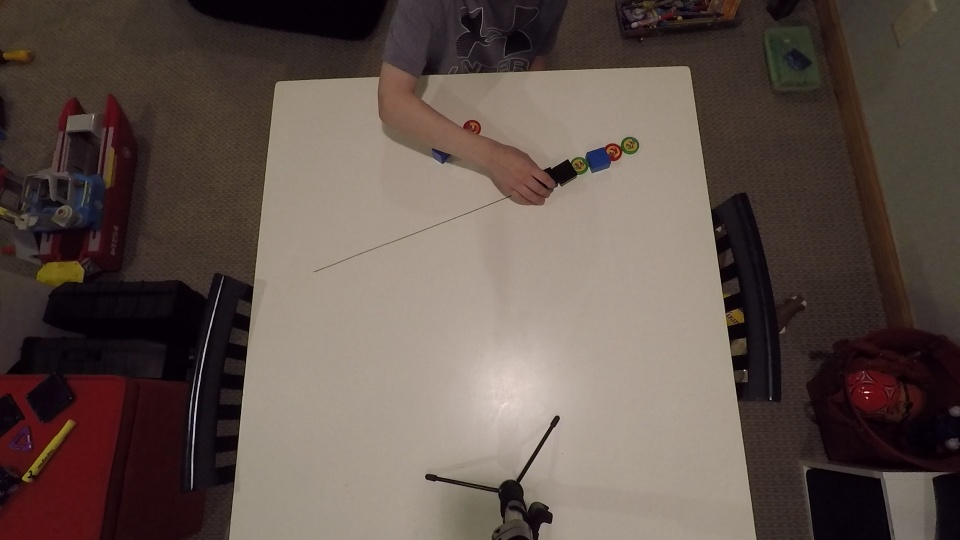
\includegraphics[width=\textwidth]{typeI.jpg} }}%
    \qquad
    \subfloat[Type II engagement]{{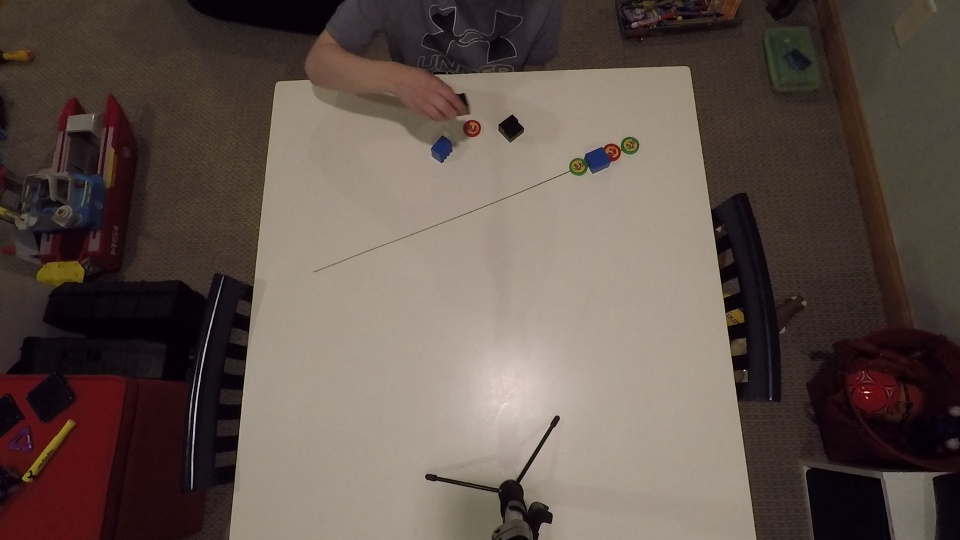
\includegraphics[width=\textwidth]{typeII.jpg} }}%
    \caption{Examples of engagements}%
    \label{engagement}%
\end{figure}
\begin{figure}%
    \centering
    \subfloat[Arranging activity setup]{{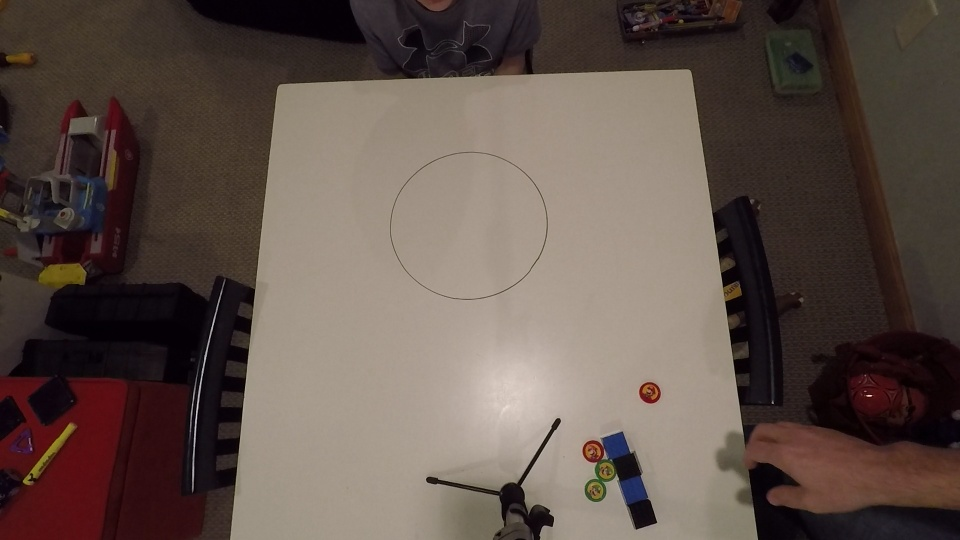
\includegraphics[width=\textwidth]{setup.jpg} }}%
    \qquad
    \subfloat[Arranging activity]{{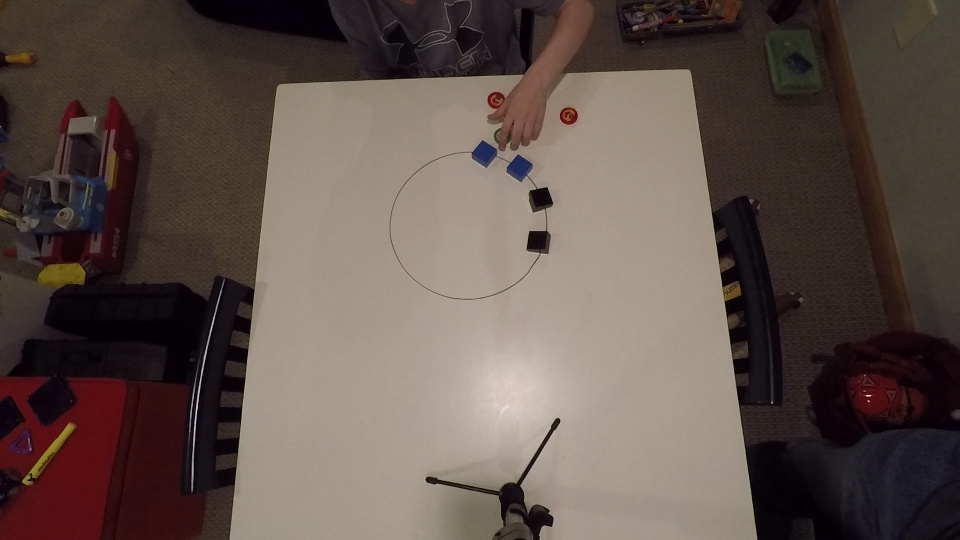
\includegraphics[width=\textwidth]{action.jpg} }}%
    \caption{Experimental setup}%
    \label{setup}%
\end{figure}
\subsubsection{Object Arrangement}
Subjects are asked to align the objects following some shape drawn on the work surface. These shapes will be predetermined and at the completion of the task, we will compute how closely the shapes are aligned with the drawn shape. Our belief is that these metrics coupled with engagments help distinguish those with ordering compulsions.

There are two shapes involved in the arrangement task and we will need metrics to define the closeness of arrangement to the template. For all shapes, we describe closeness using geometric primitives.
\begin{itemize}
	\item{Lines - using a simple Hough transform, we detect the drawn line. Next, using the midpoints of the tracked objects, we define a second line using linear regression. We use $\Theta$, the angle between the lines, and the mean squared error as metrics.\\
%	\setlength{\unitlength}{0.8cm}
%\begin{picture}(6,5)
%\thicklines
%\put(1,1){\line(1,1){4}}
%\put(1,3){\line(1,0){4}}
%\put(2,2.5){$\Theta$}
%\put(1,1){\circle*{0.75}}
%\put(2,2){\circle*{0.75}}
%\put(4.5,4.5){\circle*{0.75}}
%\caption{Metric for line arranging}
%\label{lines}
%\end{picture}
}
	\item{Circles - using a Hough circle detector, we detect the drawn circle, Then, using the midpoints of the tracked objects, we define a second circle. We define $\Delta d$, the absolute difference in the distance between the two centers, and $\Delta r = | r_{1} - r_{2} |$, the absolute difference in radii, as the metrics.
}
	\item{Spacing - Additionally, we define {\it spacing} to be the standard deviation of distance between adjacent objects in the arrangement. This is motived by the assumption that those with an ordering behavior would most likely take the extra time to make sure the objects are equally spaced.}
\end{itemize}

\subsubsection{Object Detection and Tracking}
Our setup was chosen so as to maximize our time spent in developing and refining our metrics and minimizing our time spent overcoming some of the typical difficulties in object detection. As shown in our setup, our working surface is a solid white table and the objects are simply shaped and mostly one bright color. We have chosen a simple mixture of Gaussians model for our foreground/background as there are several available in standard computer vision libraries. Despite our best efforts in the setup, there was still an issue with environmental shadows and specularities.

Our goal in tracking was to count any disappearance of an object as a type I engagement if it reappeared and overlapped with its previous location. If it moved more than that, or was tracked while visible, it was counted as a type II engagement. Since the subject's arm was not tracked, an occlusion by any part of the arm counted as an engagement. We hope to refine this in later work so that we can model the arm and hand to make more refined occlusion decisions.
\subsection{Facial Gestures}
The most frequent motor tics associated with Tourette's involve the eyes, mouth, head/neck, and nose\cite{ganos2015}. As such, we seek to recognize those parts of the body that would most discriminative in quantifying tic behavior. Our camera is setup so the axis is projected through the center of the subject's face. We place the camera far enough back so that we capture at least part of the torso so that later work might be able to capture a wider variety of non-facial tics.
\subsubsection{Blinking}
Blinking is typically an involuntary action whose function is to lubricate the eyeballs and protect from dust and other debris. The average human blinks 15-20 times per minute and spends roughly 10\% of his waking hours with closed eyes. Blinking tics as exhibited by Tourette's syndrome sufferers do not differ in rate but do differ in intensity as seen in figure \ref{blink}. Note that there is little to distinguish between the two types of blinks when seen as a single frame.

We can see in the graphs in figure \ref{ticgraph} that the blink duration during a tic is longer. This, unfortunately, is not always the case. In the graphs we have also tracked the distance between the eyebrows and the pupil and in this particular case we can see the distance decreases more severely during a tic.

\begin{figure}%
    \centering
    \subfloat[Subject blinking normally]{{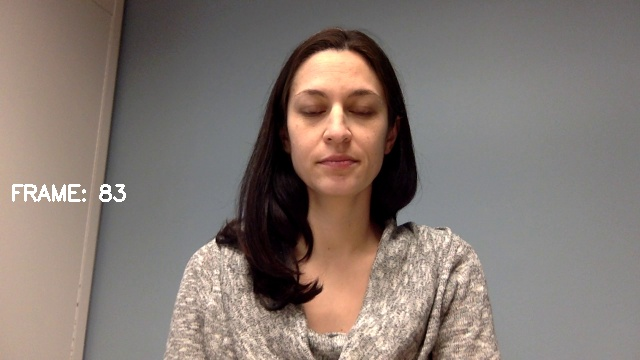
\includegraphics[width=\textwidth]{CC83.jpg} }}%
    \qquad
    \subfloat[Subject exhibiting tic behavior]{{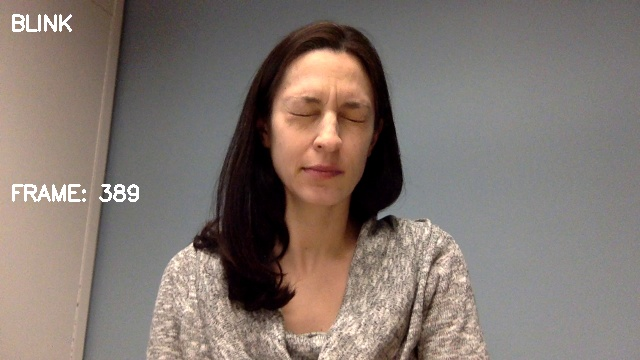
\includegraphics[width=\textwidth]{CC389.jpg} }}%
    \caption{Examples of blinking}%
    \label{blink}%
\end{figure}

\begin{figure}%
    \centering
    \subfloat[Subject not exhibiting tic behavior]{{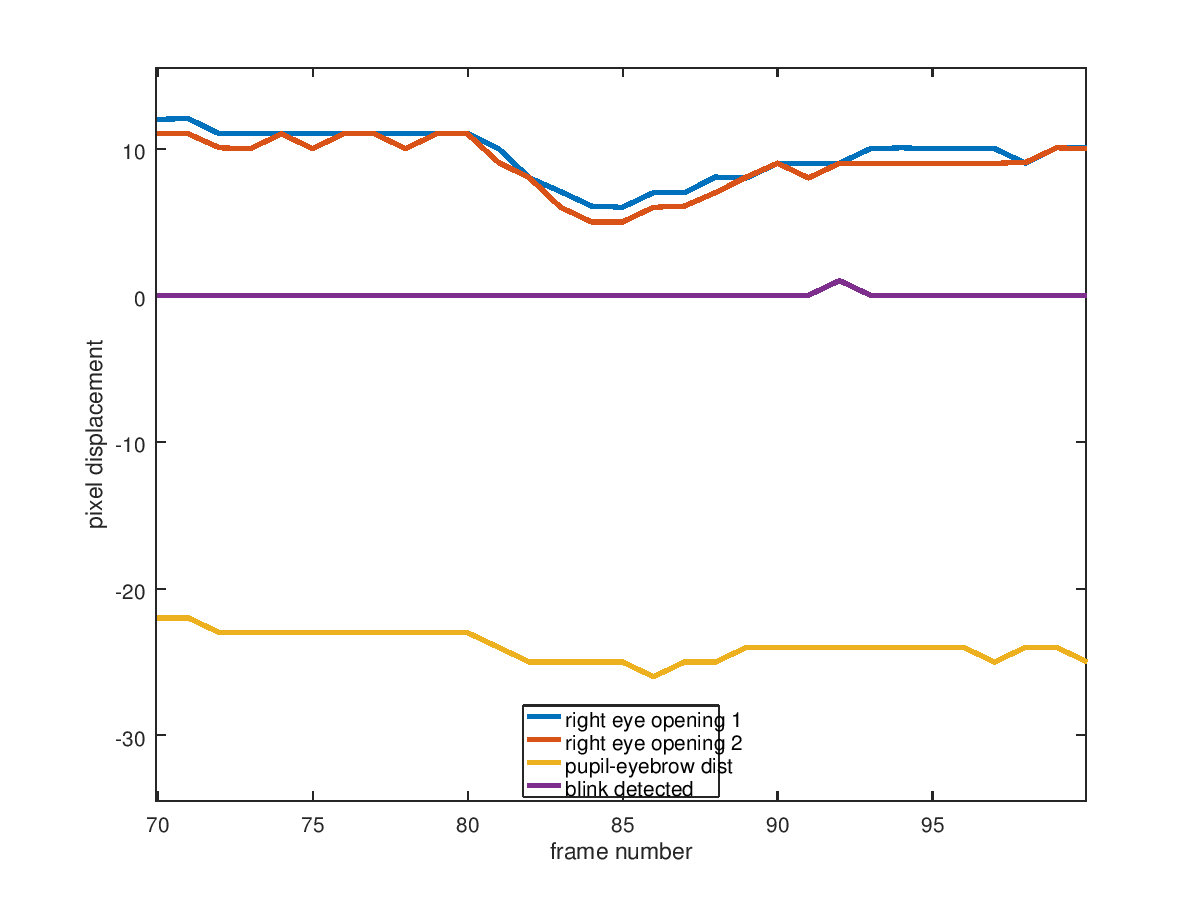
\includegraphics[width=95mm]{notic.png} }}%
    \qquad
    \subfloat[Subject exhibiting tic behavior]{{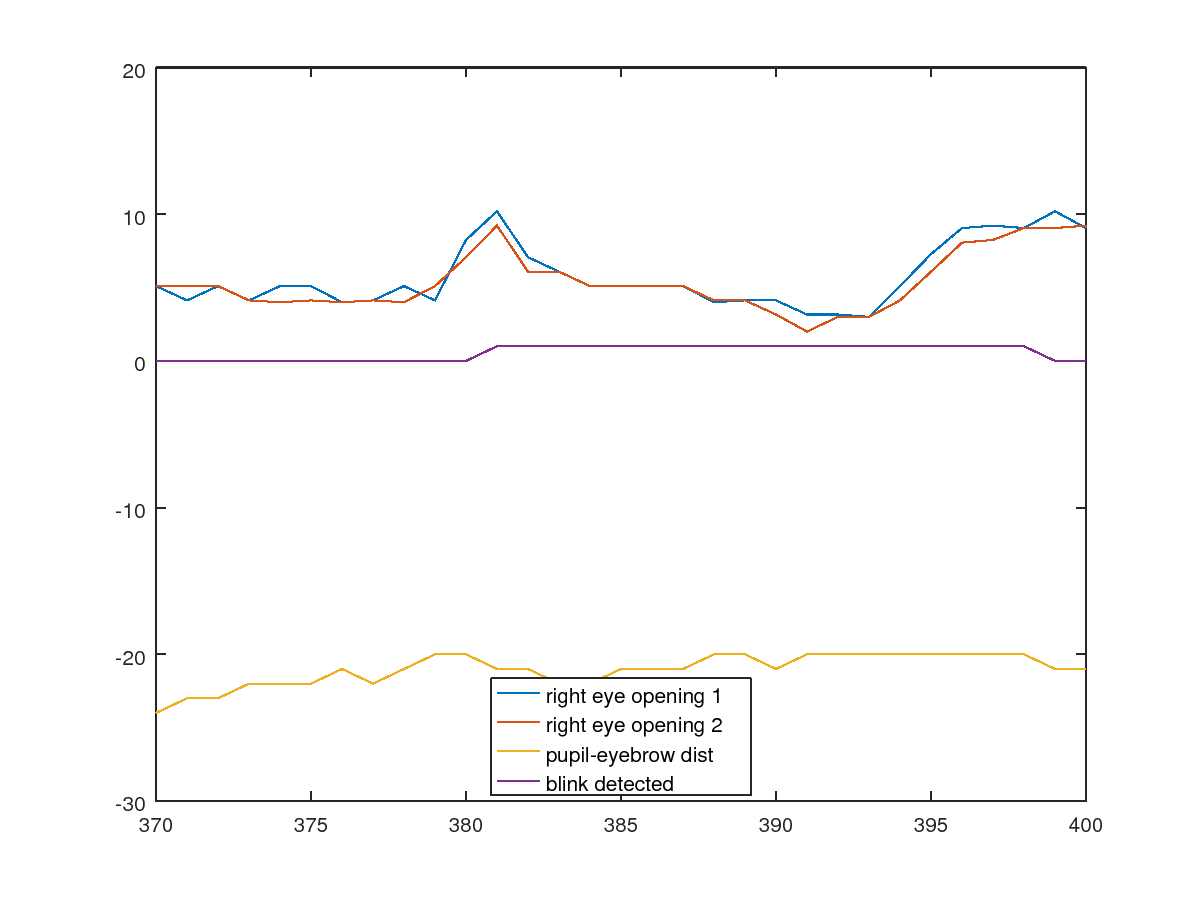
\includegraphics[width=95mm]{tic.png} }}%
    \caption{Examples of facial feature tracking during blinks}%
    \label{ticgraph}%
\end{figure}

\subsubsection{Head}
Another common manifestation in Tourette's is abnormal head motion. Sometimes this presents itself as neck stretching, where the subject's head turns and exposes one side of the neck. Other times the subject's head violently jerks to one side. In both of these cases, the gaze direction changes. Gaze direction is a commonly assessed behavior as it is present in many different disorders. In Tourette's, we expect the gaze direction to more or less stay constant and tics would be indicated by quick movements away from the center or movements that go beyond the normal expected range of motion.

\begin{figure}%
    \centering
    \subfloat[Subject gazing at camera]{{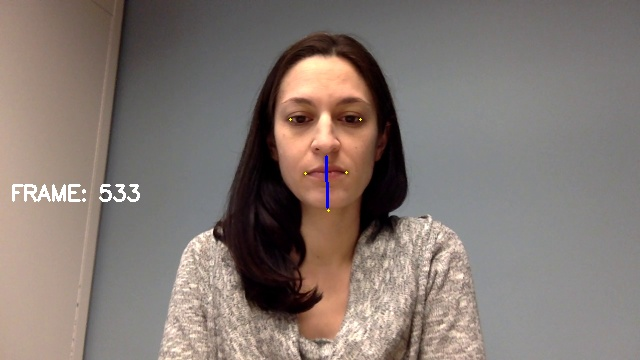
\includegraphics[width=\textwidth]{CC_gaze533.jpg} }}%
    \qquad
    \subfloat[Ssubject gazing away from camera]{{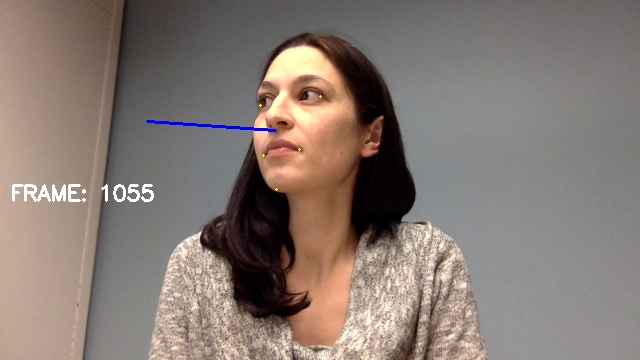
\includegraphics[width=\textwidth]{CC_gaze1055.jpg} }}%
    \caption{Examples of blinking}%
    \label{gaze}%
\end{figure}

By tracking certain feature points on a face, we can reconstruct the 3D geometry of those parts of the subject. Knowing the real world coordinates of those features(we selected eye corners, mouth corners, and tip of nose and chin with the tip of the nose as the world origin) as well as the intrinsic parameters of the camera, we can easily calculate where the subject's face is directed. Assuming that the subject will normally be gazing at the camera lens, we compute the difference angle between the gaze direction and the camera axis. However, the world coordinates of the face features will change from subject to subject and even under the best conditions are a bit imprecise.

Face feature tracking is noisy and small changes in position in even one facial feature can lead to significant changes in the gaze direction. We can see how noisy this computation is in figure \ref{gazegraph}. We will discuss better techniques in future work.
\begin{figure}%
    \centering
    \resizebox{!}{90mm}{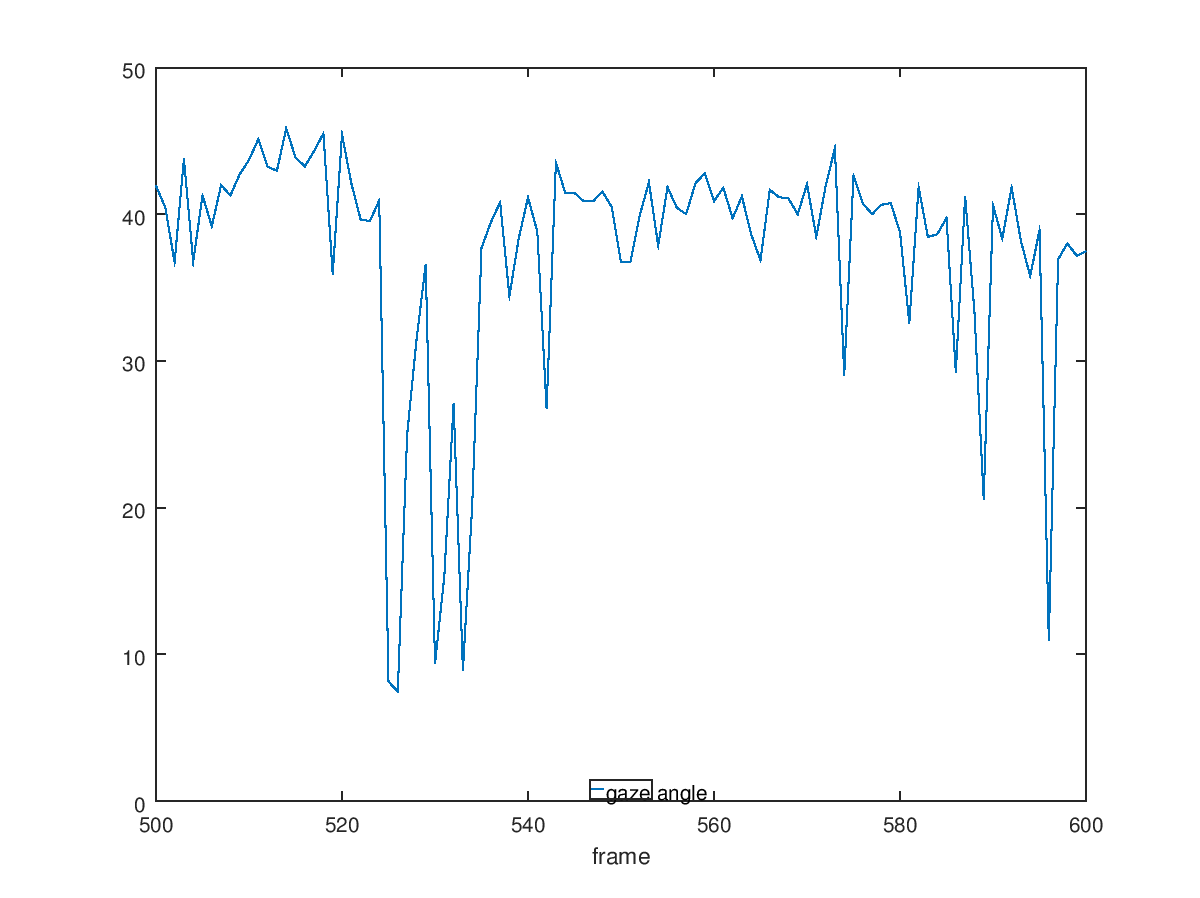
\includegraphics{headangle1.png}}
    \caption{Gaze direction of video sequnce.}
    \label{gazegraph}%
\end{figure}

\section{Proposed Work}
\subsection{Increase the data set of tic videos}
We are motivated us to start this thesis was the future applicability of the technology. We believe that being able to quantify and differentiate tic behaviors has great potential for everyday use for people suffering from TS. Not only will clinicians and researchers be able to make full use in less time of any video data, but patients will get immediate feedback on any tic suppression exercises.

Currently we have a handful of videos featuring normative subjects. For conditions in which we seek to discriminate between normal and pathological behaviors, we lack true data. At times, the subjects behaved in a way as to mimic a certain pathology. While it may have generated the appearance of real results, it does not capture the full range and nuance of the behavior. In particular, when we ask a subject to appear to tic, their action is voluntary and may not capture some of the true subtleties we may see in a true tic.

One of the goals of this work is to build discriminative tools for certain risk-factors. In order to maximize the potential utility of this tool and avoid overfitting, we need to gather video that is more representative of the general population.

For facial tics, we are partnering with Dr. Christine Conelea of the Department of Psychiatry to collect video from both the normative populations and from those who have been identified as suffering from tics. We hope this richer data set will provide the information needed to find discriminative models of tic behavior.

Additional videos will be made of the arranging task under a variety of conditions using a larger set of subjects, hopefully some who exhibit ordering compulsion. These videos will be shot under a wider range of conditions and environments to produce a more robust tracker.

We will also take advantage of already recorded video from prior research into obsessive-compulsive disorder. This videos show dyadic behavior(discussed in 5.4) which should provide for the possiblity of finding new metrics that involve more than one subject.
\subsection{Scene complexity}
Another primary goal of this work is to produce a system which can not only be used in controlled clinical settings, but also in any uncontrolled context. The real power of a system like this would be seen when it is in the hands of the patient as well as the clinician. If a patient can self-quantify his behavior, he can monitor his progress outside the clinic environment. Additionally, allowing for a simple environment for testing will open this up to more potential users.

Our initial tests in the arranging task consisted of a single top-down view. This was done as it provided the easiest initial setup for tracking. Additionally, the objects used for arranging were solid color objects on a white background. As we progress in our testing, we will add more complexity in this order.
\begin{itemize}
	\item{Multi-colored objects or objects of similar color -- we will try to make a robust tracker that can handle objects that have more varied color profiles. This wrinkle will test the robustness of tracking under occlusion.}
	\item{Varied backgrounds -- Not everyone will have access to a plain white table surface. After our tracker can handle differently-colored objects, we will alter the background to a) a darker, colored background and b) a checkered tablecloth pattern.}
	\item{Other viewpoints -- A top-down viewpoint reduces the dimensionality of the scene from 3D to 2D. We will attempt to analyze the arranging task from a 3/4 viewpoint to see if can handle occlusions from a different angle as well as motion that is not necessarily planar. Special attention will be paid to camera calibration in this section to make sure we can accurately detect circles from an arbitrary view as well as detemine object spacing in the final arrangement.}
\end{itemize}
\subsection{Hidden Markov models and Recurrent Neural Networks}
We have collected several facial features to  describe tic-like behavior but are analyzing them individually. It is more likely that these features are related and perhaps even weakly correlated. It would make sense to investigate them as a vector of features instead.

Hidden Markov models(HMM) and recurrent neural networks(RNN) have been used for activity recognition given some reduced space representation of a scene. HMMs output a sequence of labels given a sequence of observations. Using the facial features described previously as out observations, we can train a network to predict if a subject is experiencing a tic. Similarly, RNNs also create a sequence of output states given a sequence of observations with the difference being RNNs take into more than just the current observation. RNNs have shown to be better at language modeling than HMMs so we hope that we find similar results here.

Both methods are trained using a ground-truthed data set. In order to train either of these methods, we will need a larger selection of videos displaying tic and non-tic behavior.

\subsection{Dyadic interactions}
Certain behaviors may only manifest themselves in the presence of others or while doing cooperative activities. Some studies have shown a greater tendency toward hoarding or object preference during dyadic interactions. The metrics was have proposed for a single subject can be extended to multiple subjects. One could see a comparison of the solo and dyadid arranging tasks might highlight different behaviors.

Tracking two subjects adds another layer to complexity to an already difficult problem. We now are required to know which user is manipulating an object. Not only do we need to track objects, we need to track arms and hands. Because of this it will be possible for occlusions to cause multiple interaction events. Despite these hurdles, this is an interesting problem worth investigating because of its application to other fields. Being able to distinguish object/subject interaction in a busy scene is very applicable to studies of crowd surveillance.

\begin{figure}%
    \centering
    \resizebox{!}{!}{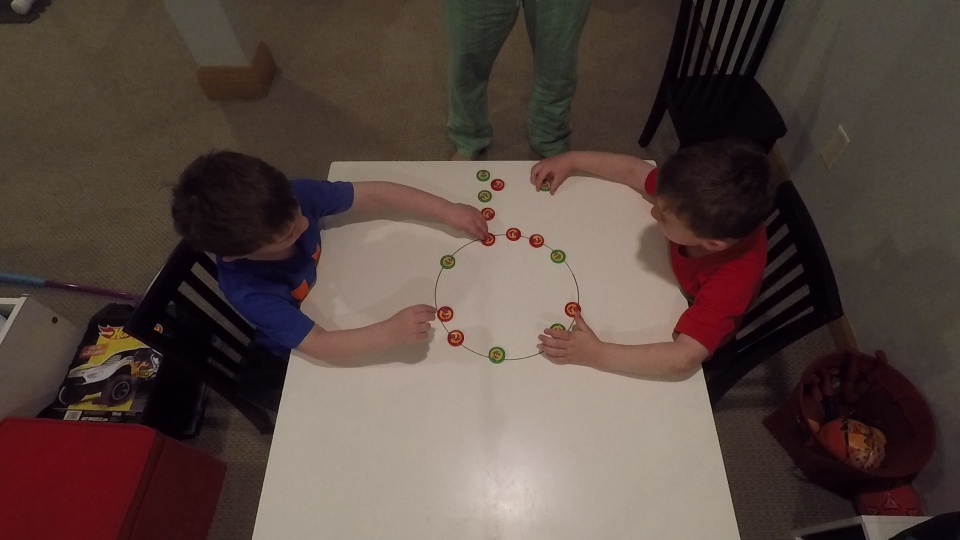
\includegraphics[width=\textwidth]{dyadic.jpg}}
    \caption{Example of the dyadic arrangment task.}
    \label{dyadic}%
\end{figure}

We will collect several videos of the arrangement task using multiple combinations of two subjects. Because of the potential difficulty of this we will limit ourselves to our initial setup of a top-down view and simple white background and remove the spacing metric. An example screenshot if shown in \ref{dyadic}.
\section{Contributions}
\subsection{Computer vision applications to medical observation}
Computer vision has been applied to many medical applications. Among the first applications was the anaylsis of medical images. Image processing has been used to detect various cancers, segment an image by tissue types, and detecting and counting white blood cells. This is an active area of research as there are still many medical images that are process manually.

Video streams have also been using in a medical context either in assisting during a procedure or in post-procedure analysis. Early work in gait recognition has been applied to the recognition of early signals of Parkinson's disease and dementia. There has been some work in the field to recognize certain behaviors to may indicate a psychiatric disorder. This thesis will explore the detection of new, subtle actions that can be quantified to assist in the evaluation of these disorders.

One of the main drawbacks of using video for medical analysis is the need to manually annotate the videos. Currently, the time requirement to do this task is too great to make general use of the videos. In fact, in many settings video recordings are never made because they will add little value a doctor/patient interaction. The ability to analyze a video automatically will increase the amount of information available to a doctor in making a diagnosis or measure disease progression.
\subsection{Human/object manipulation and tracking}
While this thesis is interesting enough in the context of mental health, tracking the manipulation of objects by a human subject is an active area of research entirely by itself. This research has been applied to work-flow optimization, scene surveillance, and even the training of robots. Much recent work has focused more on detecting and predicting interactions in static images but we see potential for our studies to be applied more broadly.

In the context of work-flow optimization, our metrics will provide insight into how often and for how long an object is interacted with which can be used as a proxy for object importance. For surveillance, we can track subjects/onjects and detect either disallowed interactions or when objects are moved beyond some physical threshold.
\section{Timeline}
A proposed timeline for the project, with a finishing data of Fall 2020, is the following:
\begin{itemize}
  \item June 2018 - December 2018: continue to gather data from a larger population
  \item January 2019 - June 2019: process videos and refine the algorithms
  \item July 2019 - January 2020: apply machine learning for behavior discrimination
  \item February 2020 - October 2020: final results and write final thesis
\end{itemize}

\pagebreak
%\bibliographystyle{../hunsrt}
\bibliography{thesis}
\end{document}
